\chapter{Analyse du système d'alerting actuel}

\section{Architecture actuelle de la chaîne d'alerting}

L'architecture étudiée repose sur un ensemble de composants AWS permettant de créer, maintenir
et diffuser des alarmes techniques autour des services déployés sur les clusters ECS. Le
fonctionnement observé peut se résumer ainsi : les changements survenant sur les services (création,
mise à jour, suppression) sont détectés via CloudTrail et EventBridge ; des fonctions Lambda
orchestrent alors la création ou la suppression d'alarmes CloudWatch ; les alarmes déclenchées
produisent des notifications qui, via un topic SNS puis une chaîne de traitement, aboutissent sur les
canaux de diffusion, principalement Slack.

\begin{figure}[h]
	\centering
	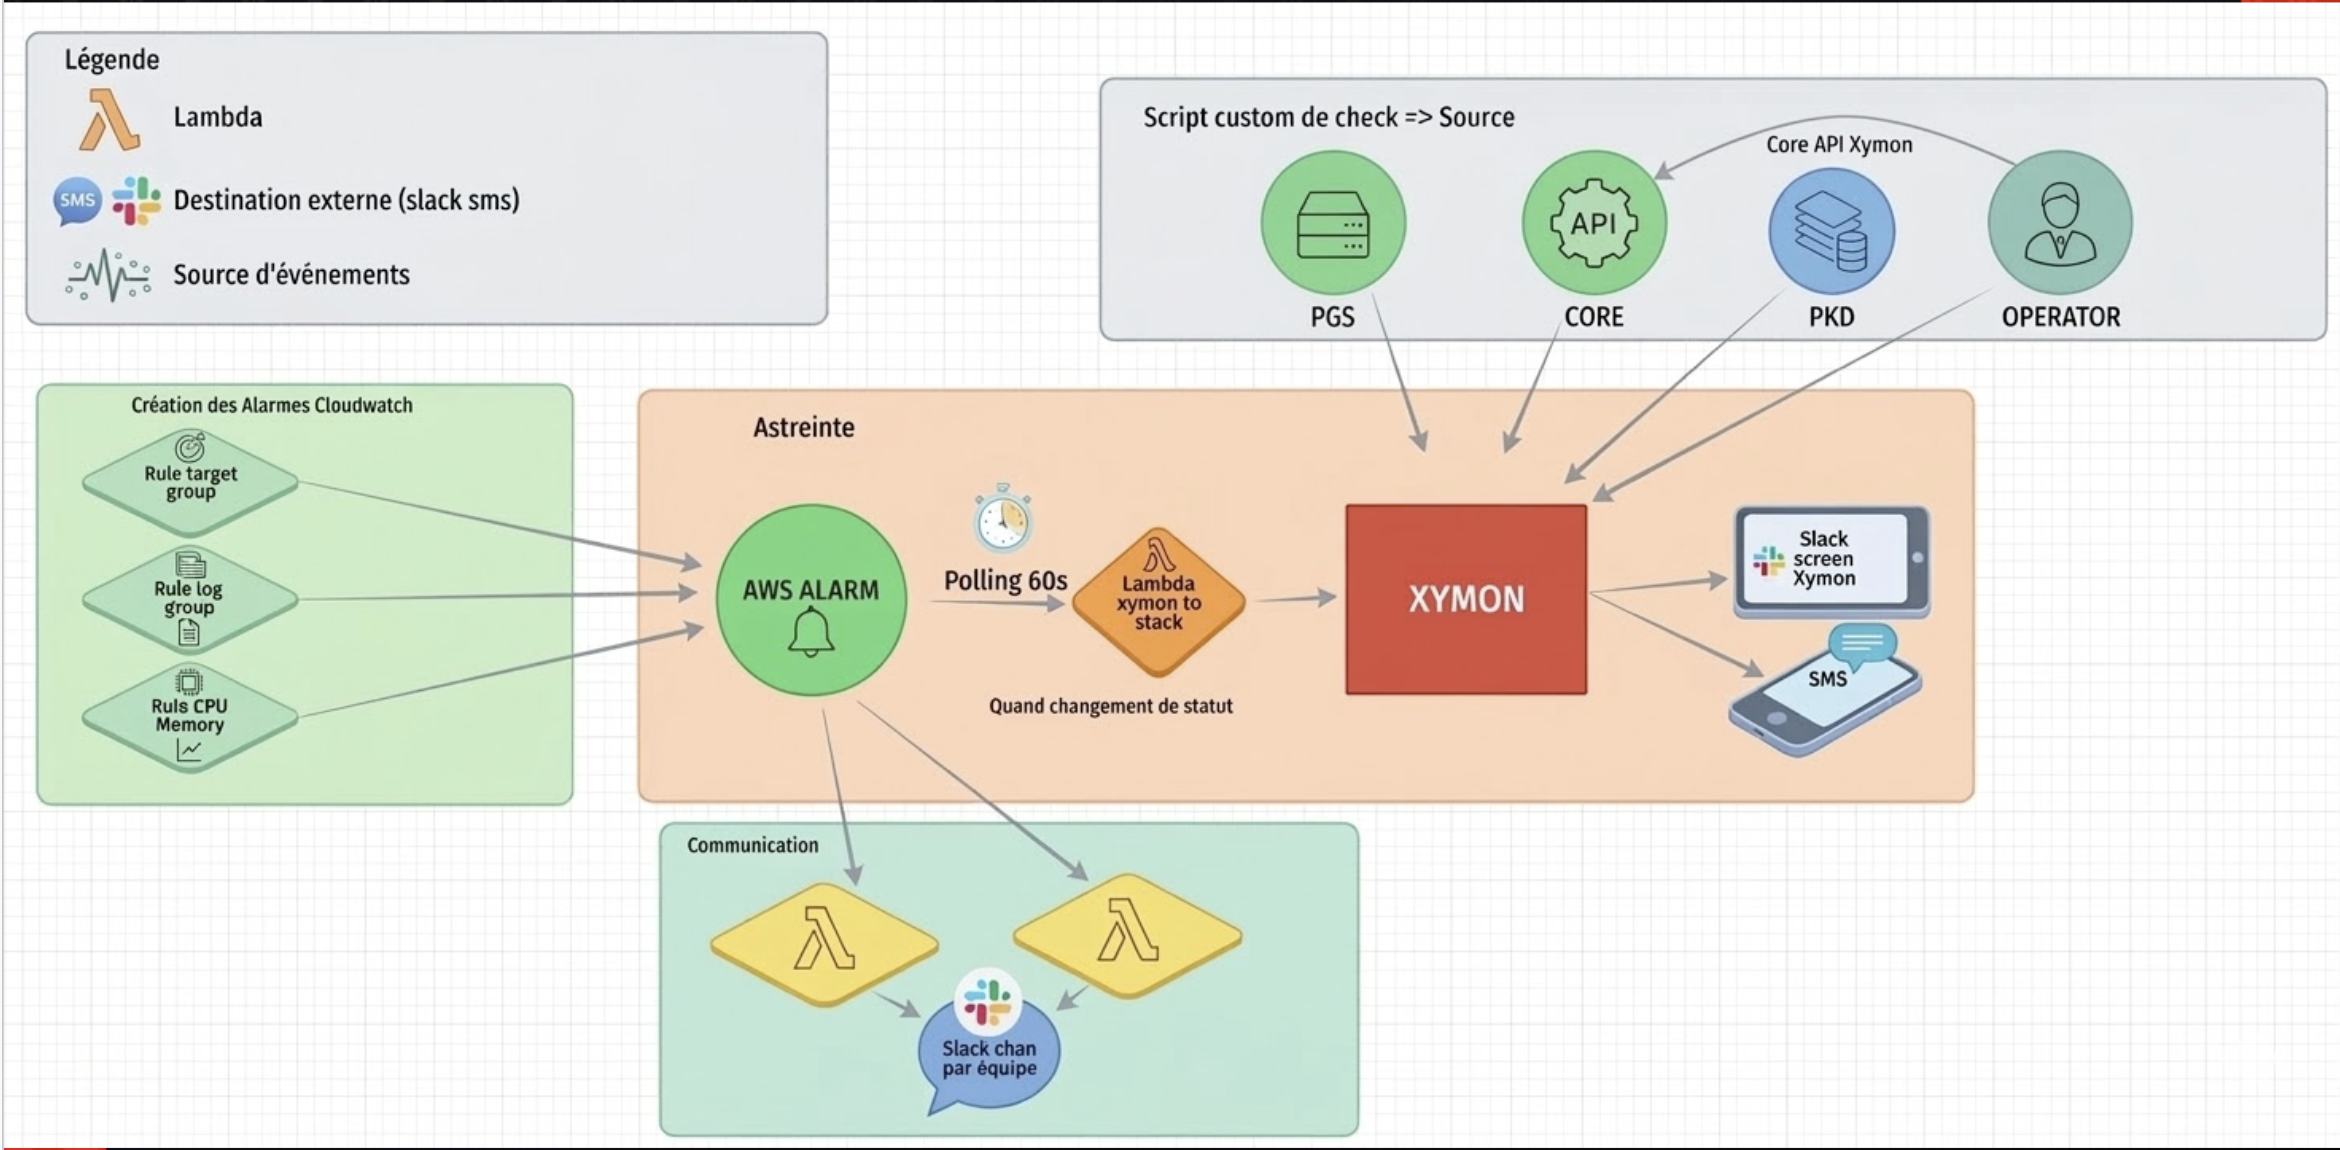
\includegraphics[width=\textwidth]{ressources-graphiques/alertingV1.png}
	\caption{Vue d'ensemble de la chaîne actuelle de création et de diffusion des alarmes}
	\label{fig:archi-alerting-actuelle}
\end{figure}
\FloatBarrier

Cette chaîne automatise entièrement la gestion des alarmes, ce qui constitue un atout indéniable,
mais elle génère aussi un niveau de complexité élevé, avec de nombreux points de configuration et un
couplage fort entre services techniques. Surtout, les alertes ainsi produites ne sont pas toujours
pertinentes pour les personnes d'astreinte.

\section{Inventaire des composants existants}

L'étude détaillée du système m'a conduit à recenser les principales fonctions Lambda qui composent
la chaîne actuelle. Chacune joue un rôle précis, mais leur enchaînement rend le système difficile à
appréhender dans son ensemble.

\begin{table}[h]
	\centering
	\caption{Récapitulatif des composants Lambda de la chaîne d'alerting actuelle}
	\label{tab:composants-lambda-actuels}
	\begin{tabular}{|p{0.35\textwidth}|p{0.55\textwidth}|}
		\hline
		\textbf{Composant (Lambda)} & \textbf{Rôle} \\
		\hline
		cloudwatch-alarms-cpu-memory & Crée les alarmes liées à la consommation de CPU et de mémoire RAM des services. \\
		\hline
		target-group-cloudwatch-alarm & Gère automatiquement les alarmes CloudWatch pour les target groups des Application Load Balancers, en fonction de tags de ressources (codes 5XX, 4XX, UnHealthyHostCount...). \\
		\hline
		cloudwatch-log-groups-stream & Gère automatiquement les filtres d'abonnement CloudWatch Logs et les alarmes pour les groupes de logs ECS, Lambda et Batch, déclenchés par les mises à jour de ressources (événements CloudTrail). \\
		\hline
		cloudwatch-logs-errors-to-slack & Écoute les événements de logs applicatifs, détermine leur pertinence (niveau error), applique des filtres anti faux-positifs, dédoublonne, journalise les métriques au format EMF et publie les logs intéressants vers SNS puis une file SQS. \\
		\hline
		rules-cloudwatch-log-groups-stream & Consomme les messages de la file SQS, construit un message Slack et détermine le canal de destination (généralement selon l'équipe). \\
		\hline
	\end{tabular}
\end{table}
\FloatBarrier

Le tag appliqué sur les target groups illustre bien la logique de configuration : chaque type d'alarme
(par exemple \texttt{HTTPCode\_Target\_5XX\_Count} ou \texttt{UnHealthyHostCount}) dispose d'un tag
d'activation booléen et d'un tag de seuil. Ce mécanisme, souple en apparence, présente en réalité de
fortes limites lorsqu'il s'agit d'introduire de la criticité ou d'harmoniser les pratiques entre équipes.

\section{Le problème de fond : alerter sur les causes plutôt que sur les conséquences}

L'étude de l'existant met en évidence une limite majeure : une partie significative des alertes est
construite autour de métriques de causes (CPU, mémoire, etc.) plutôt que des conséquenes directement
corrélés à un impact utilisateur. Concrètement, le système sait dire « la mémoire de ce conteneur est
à 80 \% » mais pas « les utilisateurs ne peuvent plus déposer d'argent ». Or c'est bien la seconde
information qui importe le plus pour l'astreinte.

Cette confusion entre causes et conséquences entraîne plusieurs effets néfastes :

\begin{itemize}
	\item des réveils d'astreinte pour des situations parfois non critiques ;
	\item une fatigue liée au volume de notifications, qui finit par émousser la vigilance ;
	\item une difficulté à identifier rapidement le service réellement en défaut.
\end{itemize}

Un pic de CPU, par exemple, peut être parfaitement normal lors d'un traitement batch et n'avoir aucun
impact sur les joueurs. À l'inverse, une latence anormale sur une API critique peut passer inaperçue si
aucune alarme ne la surveille. L'efficacité globale de la réponse à incident s'en trouve dégradée,
malgré une instrumentation technique pourtant riche.

Les alertes sur les causes sont créées automatiquement par les fonctions Lambda. 
Le système permet aussi d'alerter sur des conséquences via des scripts personnalisés, mais ces derniers sont peu utilisés et ne sont pas standardisés. 

\section{Avantages et limites de la solution existante}

Pour objectiver le diagnostic, j'ai formalisé les avantages et les inconvénients du système en place.
Cette analyse contradictoire a guidé les choix de conception de la nouvelle solution.

\begin{table}[h]
	\centering
	\caption{Points forts et limites du système d'alerting actuel}
	\label{tab:forces-limites-existant}
	\begin{tabular}{|p{0.45\textwidth}|p{0.45\textwidth}|}
		\hline
		\textbf{Points forts} & \textbf{Limites} \\
		\hline
		Création automatique des alarmes, zéro intervention manuelle pour monitorer un nouveau service &
		Perte de contrôle sur la création des alertes, aucune visibilité des équipes sur les alertes créées \\
		\hline
		Les développeurs se concentrent sur leur code &
		Chaîne trop complexe : plusieurs Lambdas avant l'envoi sur Slack \\
		\hline
		Configuration par tags sans toucher à l'infrastructure &
		Si une Lambda échoue, aucun retry : manque de visibilité \\
		\hline
		 & Beaucoup d'éléments hardcodés, code peu maintenable \\
		\hline
		 & Mêmes alertes et mêmes seuils pour tous les services \\
		\hline
		 & Impossible d'attribuer un niveau de criticité aux alertes \\
		\hline
		 & Un changement de seuil ou de nom impose de redéployer tous les services \\
		\hline
		 & Pas d'ownership des alertes par service \\
		\hline
	\end{tabular}
\end{table}
\FloatBarrier

\section{Réception des alertes par les astreintes}

Au-delà de la construction des alarmes, j'ai également étudié la manière dont les alertes parviennent
concrètement aux personnes d'astreinte. Aujourd'hui, lorsqu'une alarme CloudWatch jugée critique se
déclenche, elle provoque l'envoi d'un SMS à la personne d'astreinte, en complément de la notification
postée sur le canal Slack de l'équipe concernée.

\begin{figure}[h]
	\centering
	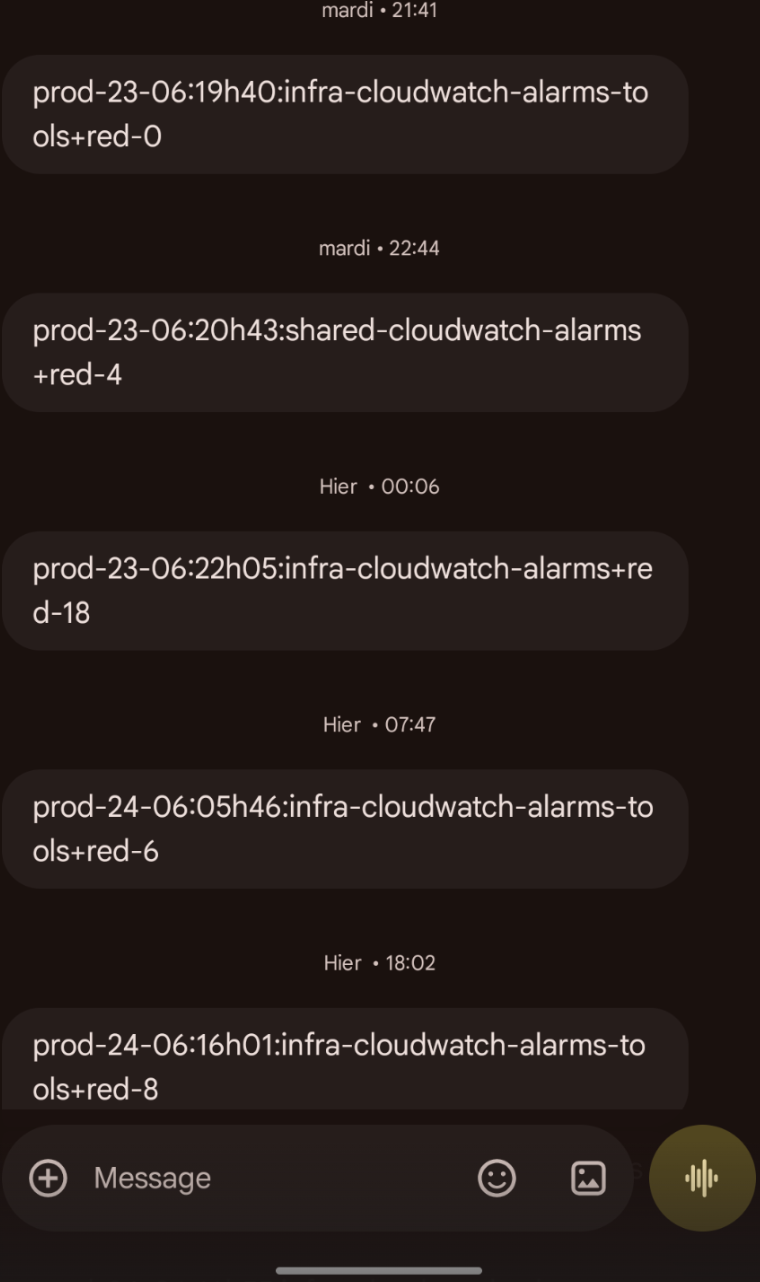
\includegraphics[width=0.35\textwidth]{ressources-graphiques/sms_astreinte.png}
	\caption{Exemple de SMS reçu par une personne d'astreinte lors du déclenchement d'une alarme}
	\label{fig:sms-astreinte}
\end{figure}
\FloatBarrier

Ce SMS se limite généralement au nom de l'alarme déclenchée, sans autre indication de contexte : ni
le niveau de criticité de l'incident, ni son impact potentiel sur les utilisateurs, ni de premières
pistes de diagnostic. La personne d'astreinte doit alors se connecter aux différents outils
(CloudWatch, dashboards, Slack) pour reconstituer le contexte et évaluer si une intervention immédiate
est nécessaire. Ce temps de latence, ajouté au réveil en pleine nuit pour des alertes qui ne sont pas
toujours critiques, contribue à dégrader l'expérience et l'efficacité de l'astreinte.

La notification déposée sur le canal Slack de l'équipe n'apporte pas davantage de contexte : elle
renvoie simplement vers la page de l'outil de supervision (Xymon) ayant généré l'alarme, comme illustré
à la figure~\ref{fig:slack-astreinte}, sans indication de criticité ni de piste de résolution.

\begin{figure}[h]
	\centering
	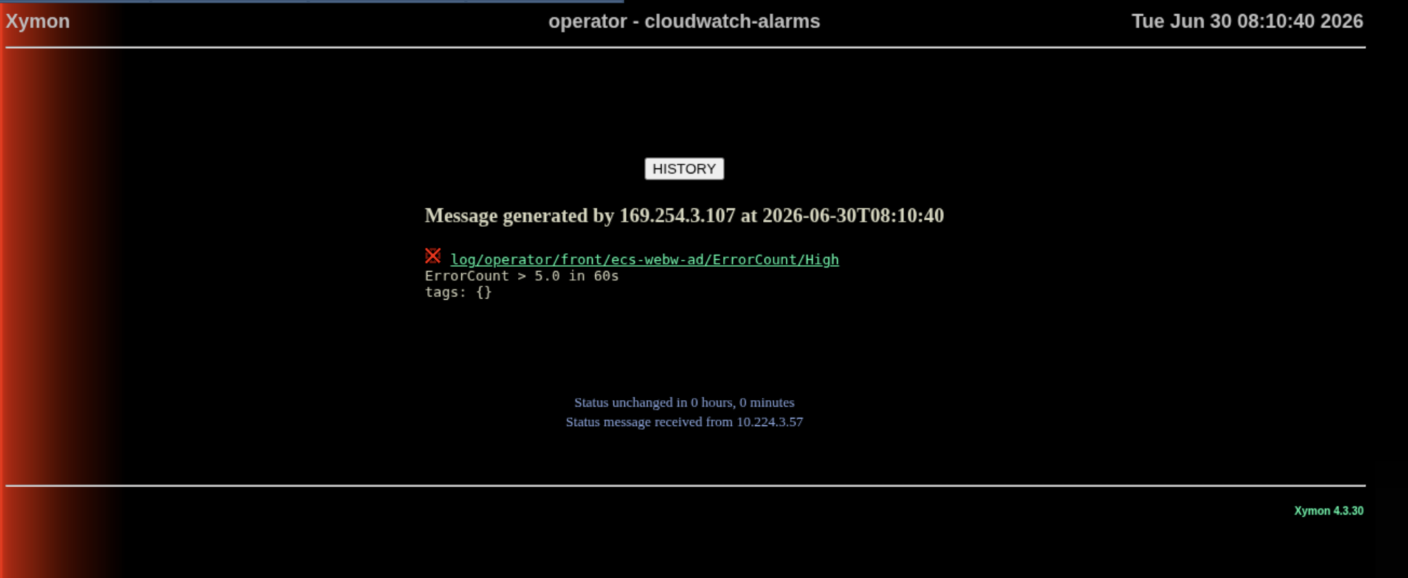
\includegraphics[width=0.8\textwidth]{ressources-graphiques/slack_astreinte.png}
	\caption{Page de supervision associée à l'alarme, consultée depuis le lien partagé sur Slack}
	\label{fig:slack-astreinte}
\end{figure}
\FloatBarrier

\section{Synthèse du diagnostic}

L'ensemble des observations précédentes permet de dresser la liste des principaux problèmes du
système d'alerting actuel :

\begin{itemize}
	\item \textbf{Absence de priorisation} : aucune notion de criticité n'est associée aux alertes, qui
	sont toutes traitées de la même manière, qu'elles nécessitent une intervention immédiate ou non ;
	\item \textbf{Manque de contexte à la réception} : les notifications (SMS, Slack) se limitent au nom
	de l'alarme déclenchée, sans information sur l'impact ni pistes de diagnostic, ce qui oblige la
	personne d'astreinte à reconstituer le contexte manuellement ;
	\item \textbf{Déclaration des alertes dispersée} : les alertes peuvent être définies à plusieurs
	endroits différents (tags de ressources, scripts personnalisés, configuration des Lambdas), sans
	guideline commune à destination des développeurs ;
	\item \textbf{Pertinence limitée des alertes} : une part importante des alertes porte sur des causes
	techniques (CPU, mémoire) plutôt que sur des conséquences réellement perçues par les utilisateurs,
	ce qui entraîne des réveils pour des situations non critiques et une fatigue d'alerte ;
	\item \textbf{Automatisation opaque} : la création des alarmes repose sur un ensemble de fonctions
	Lambda qui s'exécutent automatiquement en réaction aux événements CloudTrail, sans visibilité ni
	contrôle direct des équipes sur les alertes ainsi créées.
\end{itemize}

Ce constat justifie la définition d'un cadre de criticité formalisé, d'une méthode de déclaration des
alertes harmonisée entre équipes et d'une meilleure contextualisation des notifications, présentés
dans le chapitre suivant.
